\documentclass{article}
\usepackage[utf8]{inputenc}
\usepackage[english]{babel}
\usepackage[]{amsthm} %lets us use \begin{proof}
\usepackage[]{amssymb} %gives us the character \varnothing
\usepackage[]{setspace} %provides commands to set line spacing
\usepackage[left=0.75in, right=0.75in]{geometry}
\usepackage{hyperref}
\usepackage{xcolor}
\usepackage{amsmath}
\usepackage{enumitem}
\usepackage{graphicx}
\title{Homework 2}
\author{Son [Joe] Nguyen}
%\date{\today}

\begin{document}
%\maketitle %This command prints the title based on information entered above
\begin{center}
    \LARGE{Homework 2}\\[1em]
    \large Son [Joe] Nguyen\\[1em]
    %\large \today
\end{center}

\subsection*{Time dependent Shrodinger's equation}

\begin{equation}
    i\hbar \frac{\partial \Psi}{\partial t} = -\frac{\hbar^2}{2m} \frac{\partial^2\Psi}{\partial x^2} + V(x,t)\psi
\end{equation}
Where:
\begin{itemize}
    \item \(V(x,t)\) is the potential.
\end{itemize}

\noindent In order to get the wave function \(\Psi(x,t)\), we need to solve the Schrödinger equation (1).
If \(V\) is independent of \(t\), the Schrödinger equation can be solved by the method of separation of variables.

\begin{equation}
    \Psi(x,t) = \psi(x) \varphi(t)
\end{equation}
Where:
    \begin{itemize}
        \item \(\psi\) is the function of \(x\) alone, and \(\varphi\) is the function of \(t\) alone.
    \end{itemize}

For the separable solutions we have:

\[\frac{\partial \Psi}{\partial t} = \psi \frac{d\varphi}{dt}, \frac{\partial^2 \Psi}{\partial x^2}=\frac{d^2 \psi}{dx^2}\varphi\] 

Substitute the solutions back to equation (1). Now we have: 

\begin{equation}
    i\hbar \psi \frac{d\varphi}{dt} = -\frac{\hbar^2}{2m} \frac{d^2 \psi}{dx^2}\varphi + V(x)\psi
\end{equation}

Dividing both sides by \(\psi \varphi\):
\begin{equation}
    i\hbar \frac{1}{\varphi(t)} \frac{d\varphi}{dt} = -\frac{\hbar^2}{2m} \frac{d^2 \psi}{dx^2} \frac{1}{\psi(x)} + V(x)\psi
\end{equation}

Now the right side is the function of \(t\), and the left side is the function of \(x\). Next, we set left side equal separtion constant \(E\):

\begin{equation}
    i\hbar \frac{1}{\varphi(t)} \frac{d\varphi(t)}{dt} = E \quad \text{or} \quad \frac{d\varphi(t)}{dt} = -\frac{iE}{\hbar}\varphi(t)
\end{equation}
and:
\begin{equation}
    -\frac{\hbar^2}{2m} \frac{d^2 \psi}{dx^2} \frac{1}{\psi(x)} + V(x)\psi = E \quad \text{or} \quad -\frac{\hbar^2}{2m} \frac{\partial^2\psi}{\partial x^2} + V(x)\psi = E\psi
\end{equation}

\subsection*{Time independent Shrodinger's equation}


\begin{equation}
    -\frac{\hbar^2}{2m} \frac{\partial^2\psi}{\partial x^2} + V(x)\psi = E\psi
\end{equation}

Notice that the potential \(V\) only depends on \(x\).
\subsection*{Hamiltonian}

They are states of \emph{definite total energy}. In classical mechanics, the total energy (kinetic + potential) is called the Hamiltonian.
\begin{equation}
    H(x,p) = \frac{p^2}{2m} + V(x)
\end{equation} 

\noindent The corresponding Hamiltonian operator, obtained by the cannonical substitution \(p \rightarrow -i\hbar \frac{\partial}{\partial x}\)
\begin{align}
    &\hat{H} = -\frac{\hbar^2}{2m} \frac{\partial^2}{\partial x^2} + V(x) \\
            \Rightarrow &\hat{H} \psi = E \psi
\end{align}

The general solution is the linear combination of separable solutions. 
\[\Psi_1(x,t) = \psi_1(x)e^{-iE_1\frac{t}{\hbar}}, \Psi_2(x,t) = \psi_2(x)e^{-iE_2\frac{t}{\hbar}}, \dots\] 

There is a different wave function for each allowed energy. \newline

The general solution: 
\begin{equation}
    \Psi(x,t) =  \sum_{n=1}^{\infty}c_n \psi_n(x) e^{-iE_n\frac{t}{\hbar}}
\end{equation}

\subsection*{The Infinite Square Well}

Suppose the potential energy:

\begin{equation}
    V(x) = 
    \begin{cases}
        0 & ,0 \leq x \leq a, \\
        \infty &, \text{otherwise}
    \end{cases}
\end{equation}
Inside the well, \(V = 0\):
\[-\frac{\hbar^2}{2m}\frac{d^2\psi}{dx^2} = E\psi\]
or
\[\frac{d^2\psi}{dx^2}=-k^2\psi\]
where: 
\[k \equiv \frac{\sqrt{2mE}}{\hbar}\]
The possible values of E:
\begin{equation}
    E_n = \frac{n^2\pi^2\hbar^2}{2ma^2} = \frac{\hbar^2 k_n^2}{2m}
\end{equation}
The solution inside the well:
\begin{equation}
    \psi_n(x) = \sqrt{\frac{2}{a}}\sin(\frac{n\pi}{a}x)
\end{equation}
\subsection*{Problem 2.4}
\begin{equation*}
    \langle x \rangle = \int_{}^{} x |\Psi(x,t)|^2 dx
\end{equation*}
In the \(n\)th Stationary State:
\[|\Psi(x,t)|^2 = \Psi^* \Psi = \psi^* e^{+iE\frac{t}{\hbar}}\psi e^{-iE\frac{t}{\hbar}} = |\psi(x)|^2\]
So we have:
\[\langle x \rangle = \int_{}^{}x|\psi_n(x)|^2dx\]
from (14) we have: 
\begingroup
\allowdisplaybreaks
\begin{align}
    \langle x \rangle &= \int_{0}^{a} x \left(\sqrt{\frac{2}{a}}\sin(\frac{n\pi}{a}x)\right)^2 dx \\
                      &= \frac{2}{a} \int_{0}^{a}x \left(\sin(\frac{n\pi}{a}x)\right)^2dx \\
                      &= \frac{2}{a} \int_{0}^{a}x \left( \frac{1-cos(\alpha x)}{2} \right) dx \quad \text{where} \quad \frac{2n\pi}{a} = \alpha \\
                      &= \frac{2}{a} \left(\int_{0}^{a} \frac{x}{2}dx - \frac{1}{2}\int_{0}^{a}x\cos(\alpha x)dx\right) \\
                      &= \frac{2}{a} \left[\frac{x^2}{4}\right]^a_0 = \frac{a}{2}\\
    \langle x^2 \rangle &= \int_{0}^{a} x^2 \left(\sqrt{\frac{2}{a}}\sin(\frac{n\pi}{a}x)\right)^2 dx \\
    &= \int_{0}^{a}x^2 \left(\frac{2}{a}\sin^2(\frac{n\pi}{a}x)\right)dx \quad \text{Let \(\frac{n\pi x}{a} = y \) :} \\
    &= \int_{0}^{n\pi} \left(\frac{ay}{n\pi}\right)^2\left(\frac{2}{a}\right) \sin^2(y)\left(\frac{a}{n\pi}\right)dy \\
    &= \left(\frac{a}{n\pi}\right)^3\left(\frac{2}{a}\right) \int_{0}^{n\pi} y^2 \sin^2(y)dy \\
    &= \left(\frac{a}{n\pi}\right)^3\left(\frac{2}{a}\right) \left\{ \left[y^2 \left(\frac{y}{2}-\frac{\sin2y}{4}\right)\right]^{n\pi}_0 - \int_{0}^{n\pi} 2y \left(\frac{y}{2}-\frac{sin2y}{4}\right)dy \right\} \\
    &= \left(\frac{a}{n\pi}\right)^3\left(\frac{2}{a}\right) \left(\frac{(n\pi)^3}{6}-\frac{n\pi}{4}\right) \\
    &= a^2 \left(\frac{1}{3}-\frac{1}{2(n\pi)^2}\right) \\
    \\
    \langle \rho \rangle &= m \frac{d\langle x \rangle}{dt} = 0 \quad \text{since } \langle x \rangle \text{ is a constant} \\
    \\
  \langle \rho^2 \rangle &= \int_{0}^{a} \psi^*_n \left(\frac{\hbar}{i}\frac{d}{dx}\right)^2 \psi_n dx \\
  &= -\hbar^2 \int_{0}^{a}\psi^*_n \frac{d^2\psi_n}{dx^2}dx \\
\text{From equation (7)} \\
\langle \rho^2 \rangle &= -\hbar^2 \int_{0}^{a} \psi^2_n \left(\frac{-2mE_n}{\hbar^2}\right) \psi_n dx \\
&= 2mE_n \int_{0}^{a} |\psi_n|^2dx = 2mE_n\\
\text{From equation (13)}: \\
\langle \rho^2 \rangle &= 2m\frac{n^2\pi^2\hbar^2}{2ma^2} = \frac{n^2\pi^2\hbar^2}{a^2} \\
\sigma_x &= \sqrt{\langle x^2 \rangle - \langle x \rangle^2} = \sqrt{a^2 \left(\frac{1}{3}-\frac{1}{2(n\pi)^2}\right) - \frac{a^2}{4}} = \sqrt{\frac{a^2}{12}} \\
\sigma_p &= \sqrt{\langle \rho^2 \rangle - \langle \rho \rangle^2}= \sqrt{\frac{n^2\pi^2\hbar^2}{a^2} - 0} = \frac{n\pi\hbar}{a}
\end{align}
\endgroup

\subsection*{Problem 2.5}
\begingroup
\allowdisplaybreaks
\[\Psi(x,0)=A \left[\psi_1(x) + \psi_2(x)\right] \] 
    \begin{enumerate}[label=(\alph*)]
        \item Normalize \(\Psi(x,0)\)
        \begin{align*}
            \int_{}^{} |\Psi(x,0)|^2 dx &= 1 \\
            \int_{}^{} A^2 \left[\psi_1(x) + \psi_2(x)\right]^2 dx &= 1 \\
            A^2 \int_{}^{} \left(\psi_1(x)+\psi_2(x)\right)^*\left(\psi_1(x)+\psi_2(x)\right)dx &= 1 \\
            A^2 \int_{}^{} |\psi_1(x)|^2 + |\psi_2(x)|^2 + \psi_1^*(x)\psi_2(x) + \psi_2^*(x)\psi_1(x) dx &= 1 \\
            A^2 \left[1+1+0+0\right] &= 1 \\
            A &= \frac{1}{\sqrt{2}} \\
        \end{align*}
        \item From (11):
        \[\Psi(x,t) =  \sum_{n=1}^{\infty}c_n \psi_n(x) e^{-iE_n\frac{t}{\hbar}}\]
        when \(t = 0\):
        \[\frac{1}{\sqrt{2}}(\psi_1(x)+\psi_2(x)) = \sum_{n=1}^{\infty} c_n\psi_n(x)\]
        Now we have \(c_1=c_2=\frac{1}{\sqrt{2}}\)
        \begin{align}
            \Psi(x,t) &= \frac{1}{\sqrt{2}}\left[\psi_1(x)e^{-iE_1\frac{t}{\hbar}} + \psi_2(x)e^{-iE_2\frac{t}{\hbar}}\right] \\
            &= \frac{1}{\sqrt{2}}\left[\psi_1(x)e^{-i\frac{\pi^2\hbar}{2ma^2}t} + \psi_2(x)e^{-i\frac{4\pi^2\hbar}{2ma^2}t}\right] \\
            &= \frac{1}{\sqrt{2}} \left(\sqrt{\frac{2}{a}}\sin\left(\frac{\pi}{a}x\right)e^{-i\omega t} + \sqrt{\frac{2}{a}}\sin\left(\frac{2\pi}{a}x\right)e^{-i4\omega t}\right)\\
            &= \frac{1}{\sqrt{a}} \left(\sin \left(\frac{\pi x}{a}\right) e^{-i\omega t} + \sin\left(\frac{2\pi x}{a}\right)e^{-i 4 \omega t}\right) \\ 
            \Psi^*(x,t)\cdot\Psi(x,t) &= \frac{1}{a} \left(\sin\left(\frac{\pi x}{a}\right)e^{i \omega t} + \sin \left(\frac{2 \pi x}{a}\right)e^{i4\omega t}\right) \cdot \left(\sin \left(\frac{\pi x}{a}\right) e^{-i\omega t} + \sin\left(\frac{2\pi x}{a}\right)e^{-i 4 \omega t}\right) \\
            &= \frac{1}{a} \left(\sin^2\left(\frac{\pi x }{a}\right) + \sin^2 \left(\frac{2 \pi x}{a}\right) + \sin\left(\frac{\pi x }{a}\right)\sin\left(\frac{2 \pi x}{a}\right) \left(e^{i 3 \omega t} + e^{-i 3 \omega t}\right)\right) \\
            &= \frac{1}{a} \left(\sin^2\left(\frac{\pi x }{a}\right) + \sin^2 \left(\frac{2 \pi x}{a}\right) + 2\sin\left(\frac{\pi x}{a}\right)\sin\left(\frac{2 \pi x}{a}\right)\cos\left(3 \omega t\right)\right)
        \end{align}
        
        \item 
        \begin{align}
            \langle x \rangle &= \int_{0}^{a} x |\Psi(x,t)|^2 dx \\
            &= \int_{0}^{a} x \frac{1}{a} \left(\sin^2\left(\frac{\pi x }{a}\right) + \sin^2 \left(\frac{2 \pi x}{a}\right) + 2\sin\left(\frac{\pi x}{a}\right)\sin\left(\frac{2 \pi x}{a}\right)\cos\left(3 \omega t\right)\right) dx \\
            &= \frac{1}{a} \cos\left(3 \omega t\right) \left(\int_{0}^{a} x \sin^2\left(\frac{\pi x }{a}\right) dx + \int_{0}^{a} x \sin^2 \left(\frac{2 \pi x}{a}\right) dx + 2\int_{0}^{a} x \sin\left(\frac{\pi x}{a}\right)\sin\left(\frac{2 \pi x}{a}\right) dx\right) \\
            &= \frac{1}{a} \cos\left(3 \omega t\right) \left(\frac{a^2}{4} + \frac{a^2}{4} + 2\left(\frac{-8a^2}{9\pi^2}\right)\right)
        \end{align}
        \item 
        \begin{align}
            \langle p \rangle &= m \frac{d \langle x \rangle}{dt} \\
            &= m\frac{16 a w \sin\left(3 t w\right)}{3 \pi^2}
        \end{align}
        \item
        \[\langle H \rangle = \sum_{n=1}^{\infty} |c_n|^2E_n\]
        we have \(c_1 = c_2 = \frac{1}{\sqrt{2}}\)
        \[\langle H \rangle = \frac{1}{2}E_1 + \frac{1}{2}E_2 = \frac{5 \pi^2 \hbar^2}{4ma^2} \]
    \end{enumerate}
\endgroup
\subsection*{Problem 2.7}
\begingroup
\allowdisplaybreaks
    \begin{enumerate}[label=(\alph*)]
        \item 
        \begin{figure}[h]
            \centering
            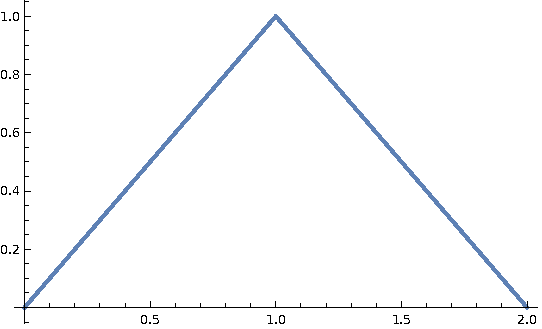
\includegraphics[width=\linewidth]{graph.pdf}
            \caption{A = 1 and a = 2}
            \label{fig:graph}
          \end{figure} 
        \[\int_{-\infty}^{\infty} |\Psi(x,0)|^2 dx = 1\] 
        \begin{align}
            \int_{0}^{\frac{a}{2}} \left(Ax)^2\right)dx + \int_{\frac{a}{2}}^{a} \left(A(a-x)^2\right)dx &= 1 \\
            \frac{a^3}{12}A^2 &= 1 \\
            A = \sqrt{\frac{12}{a^3}}
        \end{align}
        \item
        \[\Psi(x,t) =  \sum_{n=1}^{\infty}c_n \psi_n(x) e^{-iE_n\frac{t}{\hbar}}\]
        when \(t=0\)
        \[\Psi(x,0) = \sum_{n=1}^{\infty}  c_n\psi_n(x)\]
        \begin{align}
            &\int_{}^{} \sum_{n=1}^{\infty} c_n\psi_n(x)\psi_m(x)dx = \int_{}^{} \Psi(x,0)\psi_m(x)dx = \delta_{mn} \\
            \\
            c_m &= \int_{0}^{a} \Psi(x,0)\psi_m(x)dx \\
            &= \int_{0}^{\frac{a}{2}} Ax \psi_m(x)dx + \int_{\frac{a}{2}}^{a} A(a-x)\psi_m(x)dx \\
            &= A\sqrt{\frac{2}{a}}\int_{0}^{\frac{a}{2}} x sin\left(\frac{m\pi x}{a}\right)dx + A\int_{\frac{a}{2}}^{a} (a-x)\sin\left(\frac{m\pi x}{a}\right)dx \\
            &= A\sqrt{\frac{2}{a}} \left(\frac{a\left(-\frac{1}{2} a m \pi \cos\left(\frac{m \pi}{2}\right) + a \sin\left(\frac{m \pi}{2}\right)\right)}{m^2 \pi^2} \right) + A \left(\frac{a^2 \left(m \pi \cos\left(\frac{m \pi}{2}\right) + 2 \sin\left(\frac{m \pi}{2}\right)-2 \sin\left(m \pi\right)\right)}{2m^2 \pi^2}\right)\\
            &= \frac{4\sqrt{6}}{m^2 \pi^2} (-1)^{\frac{m-1}{2}}
        \end{align}
        \[\Psi(x,t)= \frac{4\sqrt{6}}{\pi^2} \sum_{n=1}^{\infty}\frac{1}{n^2}\psi_n(x)e^{-iE_n\frac{t}{\hbar}}(-1)^{\frac{n-1}{2}}\]
        
        \item The probability of \(E_n\) is equal to \(|c_n|^2\). We have: 
        \[c_n = \frac{4\sqrt{6}}{n^2 \pi^2} \quad \text{with} \quad n=1,3,5,\dots\]
        \[|c_1|^2 = \left(\frac{4\sqrt{6}}{\pi^2}\right)^2\]
        \item The expectation value of the energy:
        \begin{align}
            \langle H \rangle &= \sum_{n=1}^{\infty} |c_n|^2E_n \\
            &= \sum_{n=1,3,5,\dots}^{\infty} \left(\frac{4\sqrt{6}}{n^2 \pi^2}\right)^2 \frac{n^2 \pi^2 \hbar^2}{2ma^2} \\
            &= \frac{48\hbar^2}{\pi^2 m a^2}\sum_{n=1,3,5,\dots}^{\infty} \frac{1}{n^2}
        \end{align}
        
    \end{enumerate}
\endgroup
\subsection*{Problem 2.8}
\begingroup
\allowdisplaybreaks
Normalizing \(\Psi(x,0)\):
\begin{align}
    \int_{0}^{a} |\Psi(x,0)|^2 dx &= 1 \\
    \int_{0}^{\frac{a}{2}} |A|^2 dx &= 1 \\
    \Rightarrow A &= \sqrt{\frac{2}{a}} 
\end{align}
\\
\[\Psi(x,t) =  \sum_{n=1}^{\infty}c_n \psi_n(x) e^{-iE_n\frac{t}{\hbar}}\]
\\
Because \(\frac{\pi^2\hbar^2}{2ma^2} = E_1\). So the probability of \(E_1\) is equal to \(|c_1|^2\).
\begin{align}
    \int_{}^{} \psi_1(x)\Psi(x,0)dx &= \int_{}^{} \sum_{n=1}^{\infty} c_n \psi_n(x) \psi_1(x)dx = c_1\\
    c_1 &= \frac{2}{a} \int_{0}^{\frac{a}{2}} \sin \left(\frac{\pi}{a}x\right)dx \\
    &= \frac{2}{a} \frac{a}{\pi} = \frac{2}{\pi}\\
    &\Rightarrow |c_1|^2 = \frac{4}{\pi^2}
\end{align}

\endgroup
\end{document}
